%!TEX root = ../StatisticalCorrelations.tex

\graphicspath{{Body/Figures/Correlations/}}

\clearpage
\section{Results}


Correlation coefficients were calculated among all analyzers, all analyses, for all datasets, and between all parameters. The correlation coefficients between the \R values are presented here, since they are of the most importance\footnote{Correlation coefficients between other fit parameters are not particularly useful. One case of interest is the \R$-\phi$ correlations for a potential multi-parameter combination.}. The correlation matrix between different analyzers for the EG dataset is shown in \figref{fig:corrMatAnalyzer}. In one of the proposed combination approaches, a staged averaging method \cite{CombinationMeeting,DavidCollabTalk}, the correlation coefficients between the different reconstructions are needed. In order to determine these the \R values between the \RW T and A-Methods were averaged among the four and three different analyses respectively, before populating the scatter plots and determining the correlation coefficients\footnote{It should be noted as well that other combinations of various methods were made, one example being a weighted average of \RW AR-Methods, in order to provide a variety of correlation coefficients for corresponding types of combinations.}. The correlation matrix for the EG dataset at this reconstruction level is shown in \figref{fig:corrMatRecon}. Tables for the correlation coefficients at the analyzer level and their errors for all four datasets are given in Tables~\ref{tab:Corrs_60h_analyzer} through \ref{tab:Corrs_EG_analyzer}. Tables for the correlation coefficients at the reconstruction level and their errors for all four datasets are given in Tables ~\ref{tab:Corrs_60h_recon} through \ref{tab:Corrs_EG_recon}.



There are quite a few numbers listed throughout the tables. In order to facilitate the processing of all the information, some general summary points are as follows: 
\begin{itemize}
	\item{Correlations across the four datasets are very similar, barring some slight differences in random table entries which are usually within error of each other. An exception is for the Q-Method correlations for the 60h dataset which are around 2-3\% higher than in the rest of the datasets.}
	\item{The T-A-Methods correlation is typically around 90\%, T-Q around 50\%, T-R around 99.6\%, A-R around 90\%, and A-Q around 57\%, regardless of reconstruction.}
	\item{Errors on the analyzer level correlation coefficients are typically around 0.5\% depending on the specific correlation. In general the larger the correlation the smaller the error, just as dictated by the statistical error. Some exceptions include the errors on the Q-Method correlations which are at the 2--3\% level, and the errors on the T-R-Method correlations which are typically sub 0.1\%. In general most of the errors are at the same order as the pure statistical errors, though there are some cases where the total error is around 2 times larger.}
	\item{The T-Method correlations between \RW analyzers is typically around 98--99\%, the A-Method correlations between \RW analyzers is typically around 99\%.}
	\item{The \RE-\RW correlations are around 95\% for the T-Methods, and around 98.9\% for the A-Methods. The errors on these correlations are around 0.4 and 0.1\% respectively.}
\end{itemize}


As described in D. Sweigart's collaboration talk \cite{DavidCollabTalk}, two analyses enter the ``high-correlation'' regime when 
\begin{align}
	r_{ij} \geq \sigma_{i}/\sigma_{j},
\end{align}
where $r_{ij}$ is the correlation coefficient between two analyses $i$ and $j$, $\sigma_{i}$ and $\sigma_{j}$ are the errors of the two analyses, and $\sigma_{i} < \sigma_{j}$. In this regime, the \chisq combination approach (detailed in \refref{DavidCollabTalk}) entirely favors analysis $j$ and the combination result can even be outside the individual values of the two analyses. When comparing the correlation coefficients to these cut-offs, something like a third of so of the correlation coefficients are beyond this regime. The amount beyond the cut-off for these correlations is anywhere from small fractions of a percent to a few percent. In a good amount of these cases, this difference is within the calculated error on the coefficients. In other cases the difference cannot solely be explained by the error. If the Monte Carlo was made more like real data, with systematic effects included, then the correlations would decrease and perhaps all coefficients would drop below the cut-off (with high enough stats), though it is not known for sure.



\begin{figure}[h]
\centering
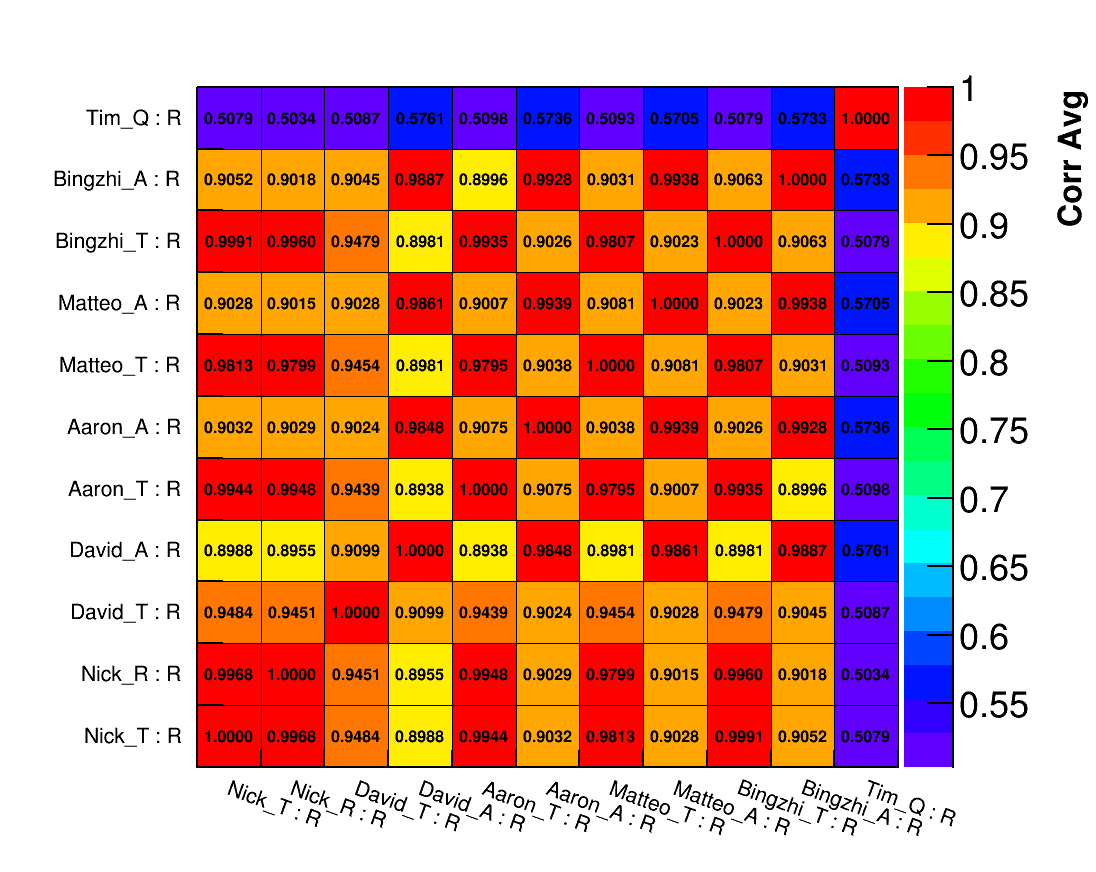
\includegraphics[width=0.85\textwidth]{Avg_CorrelationMatrix_R_R}
\caption{Correlation coefficient matrix for the \R values between different analyzers and methods for the EG dataset. Along the axes are the first names of the analyzers, the method used to fit the data, and then the fit parameter after the colon. The names here \{Nick, David, Aaron, Matteo, Bingzhi, Tim\} are the first names of the analyzers for the BU, CU, UW, EU, SJTU, and UK groups respectively. The Z axis label ``Corr Avg'' stands for the fact that the correlations are averages of the East-To-West and West-To-East variants of the Monte Carlo.}
\label{fig:corrMatAnalyzer}
\end{figure}

\begin{figure}
\centering
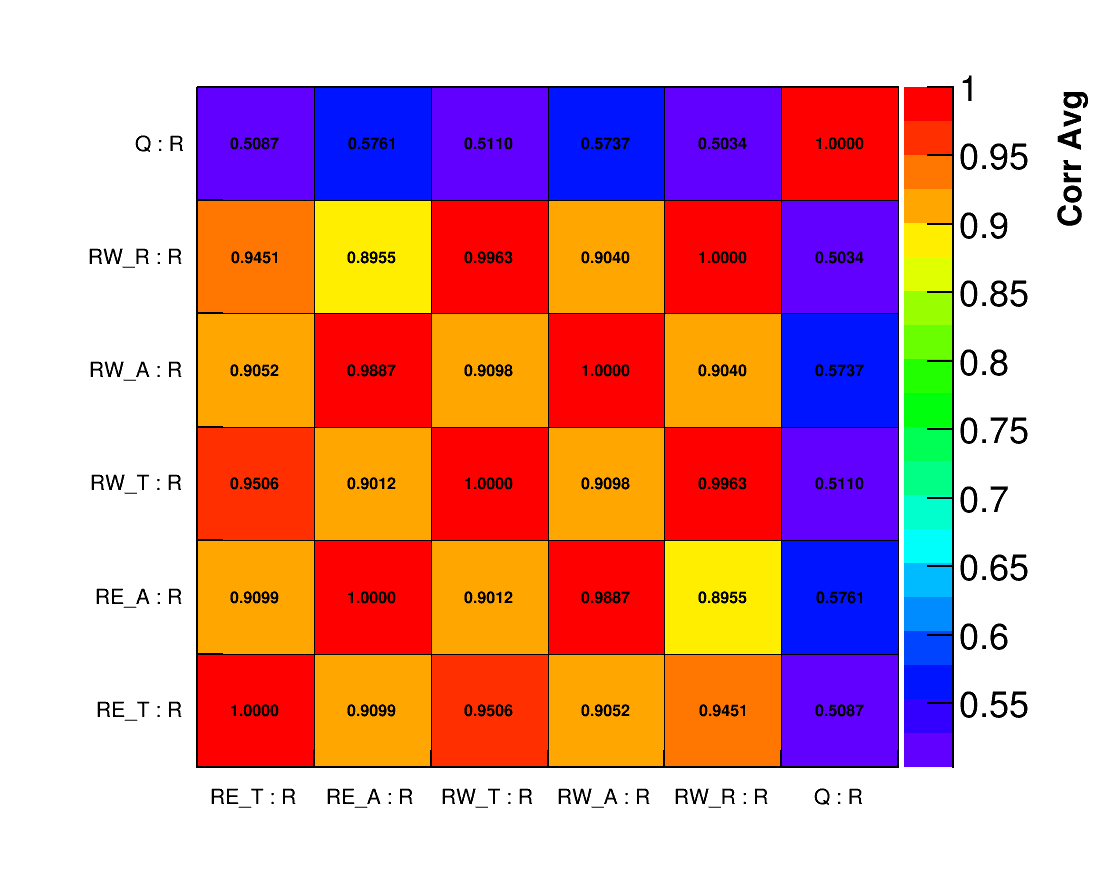
\includegraphics[width=0.85\textwidth]{Avg_Recon_CorrelationMatrix_R_R}
\caption{Correlation coefficient matrix between different reconstructions and methods for the EG dataset. Along the axes are the reconstructions, the method used to fit the data, and then the fit parameter after the colon. The \RE, R-Method, and Q-Method analyses consist of the single respective analyses. The \RW T and A-Method analysis results were averaged among the four and three different analyses respectively before calculating the coefficients. The Z axis label ``Corr Avg'' stands for the fact that the correlations are averages of the East-To-West and West-To-East variants of the Monte Carlo.}
\label{fig:corrMatRecon}
\end{figure}




% 60h

\begin{landscape}
\begin{table}
\small
\centering
\renewcommand{\arraystretch}{1.5}
\begin{tabularx}{1\linewidth}{@{\extracolsep{\fill}}lXXXXXXXXXXX}
  \toprule
  	\multicolumn{12}{c}{{\normalsize 60h Correlation Coefficients -- Analyzer Level}} \\
  \midrule
  	       & BU T & BU R & CU T & CU A & UW T & UW A & EU T & EU A & SJTU T & SJTU A & UK Q \\
  \midrule
	BU T   & 1.0000 0.0000 & 0.9964 0.0002 & 0.9445 0.0037 & 0.8992 0.0063 & 0.9935 0.0004 & 0.8977 0.0062 & 0.9783 0.0014 & 0.9014 0.0059 & 0.9992 0.0001 & 0.9050 0.0057 & 0.5279 0.0309  \\
	BU R   & 0.9964 0.0002 & 1.0000 0.0000 & 0.9418 0.0040 & 0.8969 0.0065 & 0.9943 0.0004 & 0.8987 0.0061 & 0.9776 0.0015 & 0.9008 0.0060 & 0.9956 0.0003 & 0.9023 0.0060 & 0.5256 0.0306  \\
	CU T   & 0.9445 0.0037 & 0.9418 0.0040 & 1.0000 0.0000 & 0.9043 0.0059 & 0.9395 0.0039 & 0.8933 0.0068 & 0.9399 0.0042 & 0.8963 0.0066 & 0.9436 0.0038 & 0.8992 0.0064 & 0.5248 0.0289  \\
	CU A   & 0.8992 0.0063 & 0.8969 0.0065 & 0.9043 0.0059 & 1.0000 0.0000 & 0.8972 0.0062 & 0.9840 0.0010 & 0.8999 0.0064 & 0.9855 0.0010 & 0.8985 0.0065 & 0.9892 0.0008 & 0.5926 0.0306  \\
	UW T   & 0.9935 0.0004 & 0.9943 0.0004 & 0.9395 0.0039 & 0.8972 0.0062 & 1.0000 0.0000 & 0.9065 0.0057 & 0.9771 0.0014 & 0.9025 0.0060 & 0.9928 0.0005 & 0.9022 0.0060 & 0.5324 0.0322  \\
	UW A   & 0.8977 0.0062 & 0.8987 0.0061 & 0.8933 0.0068 & 0.9840 0.0010 & 0.9065 0.0057 & 1.0000 0.0000 & 0.9016 0.0059 & 0.9933 0.0005 & 0.8971 0.0062 & 0.9916 0.0006 & 0.5927 0.0364  \\
	EU T   & 0.9783 0.0014 & 0.9776 0.0015 & 0.9399 0.0042 & 0.8999 0.0064 & 0.9771 0.0014 & 0.9016 0.0059 & 1.0000 0.0000 & 0.9091 0.0055 & 0.9775 0.0014 & 0.9041 0.0058 & 0.5406 0.0345  \\
	EU A   & 0.9014 0.0059 & 0.9008 0.0060 & 0.8963 0.0066 & 0.9855 0.0010 & 0.9025 0.0060 & 0.9933 0.0005 & 0.9091 0.0055 & 1.0000 0.0000 & 0.9006 0.0060 & 0.9934 0.0004 & 0.5928 0.0369  \\
	SJTU T & 0.9992 0.0001 & 0.9956 0.0003 & 0.9436 0.0038 & 0.8985 0.0065 & 0.9928 0.0005 & 0.8971 0.0062 & 0.9775 0.0014 & 0.9006 0.0060 & 1.0000 0.0000 & 0.9058 0.0057 & 0.5271 0.0305  \\
	SJTU A & 0.9050 0.0057 & 0.9023 0.0060 & 0.8992 0.0064 & 0.9892 0.0008 & 0.9022 0.0060 & 0.9916 0.0006 & 0.9041 0.0058 & 0.9934 0.0004 & 0.9058 0.0057 & 1.0000 0.0000 & 0.5893 0.0343  \\
	UK Q   & 0.5279 0.0309 & 0.5256 0.0306 & 0.5248 0.0289 & 0.5926 0.0306 & 0.5324 0.0322 & 0.5927 0.0364 & 0.5406 0.0345 & 0.5928 0.0369 & 0.5271 0.0305 & 0.5893 0.0343 & 1.0000 0.0000  \\
  \bottomrule
\end{tabularx}
\caption[]{Correlation coefficients between \R values for the 60h dataset, at the analyzer level. In each table cell, the top number is the correlation coefficient and the bottom number is the error on the coefficient.}
\label{tab:Corrs_60h_analyzer}
\end{table}
\end{landscape}

% HK

\begin{landscape}
\begin{table}
\small
\centering
\renewcommand{\arraystretch}{1.5}
\begin{tabularx}{1\linewidth}{@{\extracolsep{\fill}}lXXXXXXXXXXX}
  \toprule
  	\multicolumn{12}{c}{{\normalsize HK Correlation Coefficients -- Analyzer Level}} \\
  \midrule
  	       & BU T & BU R & CU T & CU A & UW T & UW A & EU T & EU A & SJTU T & SJTU A & UK Q \\
  \midrule
	BU T   & 1.0000 0.0000 & 0.9967 0.0002 & 0.9469 0.0040 & 0.8924 0.0077 & 0.9939 0.0005 & 0.8938 0.0065 & 0.9799 0.0017 & 0.8946 0.0071 & 0.9992 0.0001 & 0.8978 0.0070 & 0.4982 0.0245  \\
	BU R   & 0.9967 0.0002 & 1.0000 0.0000 & 0.9439 0.0042 & 0.8907 0.0081 & 0.9943 0.0005 & 0.8955 0.0065 & 0.9785 0.0017 & 0.8948 0.0072 & 0.9958 0.0003 & 0.8959 0.0072 & 0.4959 0.0249  \\
	CU T   & 0.9469 0.0040 & 0.9439 0.0042 & 1.0000 0.0000 & 0.8968 0.0068 & 0.9408 0.0046 & 0.8858 0.0068 & 0.9409 0.0038 & 0.8865 0.0068 & 0.9458 0.0042 & 0.8900 0.0067 & 0.4913 0.0266  \\
	CU A   & 0.8924 0.0077 & 0.8907 0.0081 & 0.8968 0.0068 & 1.0000 0.0000 & 0.8872 0.0089 & 0.9839 0.0014 & 0.8900 0.0071 & 0.9846 0.0011 & 0.8913 0.0079 & 0.9892 0.0008 & 0.5635 0.0256  \\
	UW T   & 0.9939 0.0005 & 0.9943 0.0005 & 0.9408 0.0046 & 0.8872 0.0089 & 1.0000 0.0000 & 0.8993 0.0064 & 0.9776 0.0025 & 0.8928 0.0077 & 0.9930 0.0005 & 0.8920 0.0080 & 0.5015 0.0238  \\
	UW A   & 0.8938 0.0065 & 0.8955 0.0065 & 0.8858 0.0068 & 0.9839 0.0014 & 0.8993 0.0064 & 1.0000 0.0000 & 0.8943 0.0064 & 0.9935 0.0007 & 0.8928 0.0067 & 0.9918 0.0007 & 0.5642 0.0245  \\
	EU T   & 0.9799 0.0017 & 0.9785 0.0017 & 0.9409 0.0038 & 0.8900 0.0071 & 0.9776 0.0025 & 0.8943 0.0064 & 1.0000 0.0000 & 0.8998 0.0062 & 0.9791 0.0018 & 0.8949 0.0066 & 0.5066 0.0236  \\
	EU A   & 0.8946 0.0071 & 0.8948 0.0072 & 0.8865 0.0068 & 0.9846 0.0011 & 0.8928 0.0077 & 0.9935 0.0007 & 0.8998 0.0062 & 1.0000 0.0000 & 0.8936 0.0073 & 0.9935 0.0004 & 0.5637 0.0247  \\
	SJTU T & 0.9992 0.0001 & 0.9958 0.0003 & 0.9458 0.0042 & 0.8913 0.0079 & 0.9930 0.0005 & 0.8928 0.0067 & 0.9791 0.0018 & 0.8936 0.0073 & 1.0000 0.0000 & 0.8984 0.0071 & 0.4987 0.0245  \\
	SJTU A & 0.8978 0.0070 & 0.8959 0.0072 & 0.8900 0.0067 & 0.9892 0.0008 & 0.8920 0.0080 & 0.9918 0.0007 & 0.8949 0.0066 & 0.9935 0.0004 & 0.8984 0.0071 & 1.0000 0.0000 & 0.5612 0.0259  \\
	UK Q   & 0.4982 0.0245 & 0.4959 0.0249 & 0.4913 0.0266 & 0.5635 0.0256 & 0.5015 0.0238 & 0.5642 0.0245 & 0.5066 0.0236 & 0.5637 0.0247 & 0.4987 0.0245 & 0.5612 0.0259 & 1.0000 0.0000  \\
  \bottomrule
\end{tabularx}
\caption[]{Correlation coefficients between \R values for the HK dataset, at the analyzer level. In each table cell, the top number is the correlation coefficient and the bottom number is the error on the coefficient.}
\label{tab:Corrs_HK_analyzer}
\end{table}
\end{landscape}

% 9d

\begin{landscape}
\begin{table}
\small
\centering
\renewcommand{\arraystretch}{1.5}
\begin{tabularx}{1\linewidth}{@{\extracolsep{\fill}}lXXXXXXXXXXX}
  \toprule
  	\multicolumn{12}{c}{{\normalsize 9d Correlation Coefficients -- Analyzer Level}} \\
  \midrule
  	       & BU T & BU R & CU T & CU A & UW T & UW A & EU T & EU A & SJTU T & SJTU A & UK Q \\
  \midrule
	BU T   & 1.0000 0.0000 & 0.9965 0.0004 & 0.9445 0.0037 & 0.8912 0.0109 & 0.9939 0.0006 & 0.8935 0.0086 & 0.9787 0.0023 & 0.8952 0.0103 & 0.9993 0.0001 & 0.8983 0.0094 & 0.4936 0.0261  \\
	BU R   & 0.9965 0.0004 & 1.0000 0.0000 & 0.9414 0.0040 & 0.8885 0.0118 & 0.9944 0.0005 & 0.8944 0.0088 & 0.9782 0.0017 & 0.8945 0.0105 & 0.9958 0.0004 & 0.8957 0.0099 & 0.4888 0.0265  \\
	CU T   & 0.9445 0.0037 & 0.9414 0.0040 & 1.0000 0.0000 & 0.9002 0.0064 & 0.9392 0.0045 & 0.8905 0.0066 & 0.9419 0.0037 & 0.8906 0.0068 & 0.9438 0.0039 & 0.8944 0.0066 & 0.5000 0.0248  \\
	CU A   & 0.8912 0.0109 & 0.8885 0.0118 & 0.9002 0.0064 & 1.0000 0.0000 & 0.8861 0.0122 & 0.9833 0.0011 & 0.8904 0.0088 & 0.9840 0.0011 & 0.8903 0.0111 & 0.9886 0.0009 & 0.5710 0.0213  \\
	UW T   & 0.9939 0.0006 & 0.9944 0.0005 & 0.9392 0.0045 & 0.8861 0.0122 & 1.0000 0.0000 & 0.8990 0.0091 & 0.9770 0.0018 & 0.8931 0.0117 & 0.9931 0.0007 & 0.8929 0.0109 & 0.4999 0.0270  \\
	UW A   & 0.8935 0.0086 & 0.8944 0.0088 & 0.8905 0.0066 & 0.9833 0.0011 & 0.8990 0.0091 & 1.0000 0.0000 & 0.8966 0.0070 & 0.9932 0.0005 & 0.8926 0.0088 & 0.9923 0.0005 & 0.5750 0.0214  \\
	EU T   & 0.9787 0.0023 & 0.9782 0.0017 & 0.9419 0.0037 & 0.8904 0.0088 & 0.9770 0.0018 & 0.8966 0.0070 & 1.0000 0.0000 & 0.9021 0.0082 & 0.9778 0.0023 & 0.8974 0.0081 & 0.4992 0.0241  \\
	EU A   & 0.8952 0.0103 & 0.8945 0.0105 & 0.8906 0.0068 & 0.9840 0.0011 & 0.8931 0.0117 & 0.9932 0.0005 & 0.9021 0.0082 & 1.0000 0.0000 & 0.8944 0.0104 & 0.9940 0.0004 & 0.5698 0.0214  \\
	SJTU T & 0.9993 0.0001 & 0.9958 0.0004 & 0.9438 0.0039 & 0.8903 0.0111 & 0.9931 0.0007 & 0.8926 0.0088 & 0.9778 0.0023 & 0.8944 0.0104 & 1.0000 0.0000 & 0.8988 0.0095 & 0.4913 0.0263  \\
	SJTU A & 0.8983 0.0094 & 0.8957 0.0099 & 0.8944 0.0066 & 0.9886 0.0009 & 0.8929 0.0109 & 0.9923 0.0005 & 0.8974 0.0081 & 0.9940 0.0004 & 0.8988 0.0095 & 1.0000 0.0000 & 0.5651 0.0216  \\
	UK Q   & 0.4936 0.0261 & 0.4888 0.0265 & 0.5000 0.0248 & 0.5710 0.0213 & 0.4999 0.0270 & 0.5750 0.0214 & 0.4992 0.0241 & 0.5698 0.0214 & 0.4913 0.0263 & 0.5651 0.0216 & 1.0000 0.0000  \\
  \bottomrule
\end{tabularx}
\caption[]{Correlation coefficients between \R values for the 9d dataset, at the analyzer level. In each table cell, the top number is the correlation coefficient and the bottom number is the error on the coefficient.}
\label{tab:Corrs_9d_analyzer}
\end{table}
\end{landscape}

% EG

\begin{landscape}
\begin{table}
\small
\centering
\renewcommand{\arraystretch}{1.5}
\begin{tabularx}{1\linewidth}{@{\extracolsep{\fill}}lXXXXXXXXXXX}
  \toprule
  	\multicolumn{12}{c}{{\normalsize EG Correlation Coefficients -- Analyzer Level}} \\
  \midrule
  	       & BU T & BU R & CU T & CU A & UW T & UW A & EU T & EU A & SJTU T & SJTU A & UK Q \\
  \midrule
	BU T   & 1.0000 0.0000 & 0.9968 0.0002 & 0.9484 0.0040 & 0.8988 0.0113 & 0.9944 0.0006 & 0.9032 0.0097 & 0.9813 0.0013 & 0.9028 0.0107 & 0.9991 0.0001 & 0.9052 0.0108 & 0.5079 0.0275  \\
	BU R   & 0.9968 0.0002 & 1.0000 0.0000 & 0.9451 0.0045 & 0.8955 0.0122 & 0.9948 0.0007 & 0.9029 0.0107 & 0.9799 0.0015 & 0.9015 0.0115 & 0.9960 0.0003 & 0.9018 0.0118 & 0.5034 0.0275  \\
	CU T   & 0.9484 0.0040 & 0.9451 0.0045 & 1.0000 0.0000 & 0.9099 0.0064 & 0.9439 0.0042 & 0.9024 0.0064 & 0.9454 0.0049 & 0.9028 0.0064 & 0.9479 0.0038 & 0.9045 0.0063 & 0.5087 0.0270  \\
	CU A   & 0.8988 0.0113 & 0.8955 0.0122 & 0.9099 0.0064 & 1.0000 0.0000 & 0.8938 0.0121 & 0.9848 0.0011 & 0.8981 0.0124 & 0.9861 0.0010 & 0.8981 0.0113 & 0.9887 0.0010 & 0.5761 0.0230  \\
	UW T   & 0.9944 0.0006 & 0.9948 0.0007 & 0.9439 0.0042 & 0.8938 0.0121 & 1.0000 0.0000 & 0.9075 0.0099 & 0.9795 0.0017 & 0.9007 0.0115 & 0.9935 0.0007 & 0.8996 0.0120 & 0.5098 0.0274  \\
	UW A   & 0.9032 0.0097 & 0.9029 0.0107 & 0.9024 0.0064 & 0.9848 0.0011 & 0.9075 0.0099 & 1.0000 0.0000 & 0.9038 0.0108 & 0.9939 0.0006 & 0.9026 0.0096 & 0.9928 0.0006 & 0.5736 0.0233  \\
	EU T   & 0.9813 0.0013 & 0.9799 0.0015 & 0.9454 0.0049 & 0.8981 0.0124 & 0.9795 0.0017 & 0.9038 0.0108 & 1.0000 0.0000 & 0.9081 0.0113 & 0.9807 0.0014 & 0.9031 0.0115 & 0.5093 0.0267  \\
	EU A   & 0.9028 0.0107 & 0.9015 0.0115 & 0.9028 0.0064 & 0.9861 0.0010 & 0.9007 0.0115 & 0.9939 0.0006 & 0.9081 0.0113 & 1.0000 0.0000 & 0.9023 0.0107 & 0.9938 0.0005 & 0.5705 0.0234  \\
	SJTU T & 0.9991 0.0001 & 0.9960 0.0003 & 0.9479 0.0038 & 0.8981 0.0113 & 0.9935 0.0007 & 0.9026 0.0096 & 0.9807 0.0014 & 0.9023 0.0107 & 1.0000 0.0000 & 0.9063 0.0106 & 0.5079 0.0278  \\
	SJTU A & 0.9052 0.0108 & 0.9018 0.0118 & 0.9045 0.0063 & 0.9887 0.0010 & 0.8996 0.0120 & 0.9928 0.0006 & 0.9031 0.0115 & 0.9938 0.0005 & 0.9063 0.0106 & 1.0000 0.0000 & 0.5733 0.0231  \\
	UK Q   & 0.5079 0.0275 & 0.5034 0.0275 & 0.5087 0.0270 & 0.5761 0.0230 & 0.5098 0.0274 & 0.5736 0.0233 & 0.5093 0.0267 & 0.5705 0.0234 & 0.5079 0.0278 & 0.5733 0.0231 & 1.0000 0.0000  \\
  \bottomrule
\end{tabularx}
\caption[]{Correlation coefficients between \R values for the EG dataset, at the analyzer level. In each table cell, the top number is the correlation coefficient and the bottom number is the error on the coefficient.}
\label{tab:Corrs_EG_analyzer}
\end{table}
\end{landscape}



% recon correlations below here

% \subsection{Reconstruction Level Correlations}
% \label{sub:reconcorrelations}

\clearpage

\begin{table}[t]
\setlength\tabcolsep{15pt}
\footnotesize
\centering
\renewcommand{\arraystretch}{1.4}
\begin{tabularx}{0.8\linewidth}{@{\extracolsep{\fill}}lXXXXXX}
  \toprule
  	\multicolumn{7}{c}{{\normalsize 60h Correlation Coefficients -- Recon. Level}} \\
  \midrule
  	       & RE T & RE A & RW T & RW A & RW R & \quad Q \\
  \midrule
	RE T   & 1.0000 0.0000 & 0.9043 0.0059 & 0.9467 0.0036 & 0.8984 0.0065 & 0.9418 0.0040 & 0.5248 0.0289  \\
	RE A   & 0.9043 0.0059 & 1.0000 0.0000 & 0.9033 0.0060 & 0.9886 0.0008 & 0.8969 0.0065 & 0.5926 0.0306  \\
	RW T   & 0.9467 0.0036 & 0.9033 0.0060 & 1.0000 0.0000 & 0.9097 0.0055 & 0.9961 0.0003 & 0.5348 0.0320  \\
	RW A   & 0.8984 0.0065 & 0.9886 0.0008 & 0.9097 0.0055 & 1.0000 0.0000 & 0.9028 0.0059 & 0.5930 0.0359  \\
	RW R   & 0.9418 0.0040 & 0.8969 0.0065 & 0.9961 0.0003 & 0.9028 0.0059 & 1.0000 0.0000 & 0.5256 0.0306  \\
	Q      & 0.5248 0.0289 & 0.5926 0.0306 & 0.5348 0.0320 & 0.5930 0.0359 & 0.5256 0.0306 & 1.0000 0.0000  \\
  \bottomrule
\end{tabularx}
\caption[]{Correlation coefficients between \R values for the 60h dataset, at the reconstruction level, after the \RW T-Method and A-Method \R values were averaged among the different analyzers. In each table cell, the top number is the correlation coefficient and the bottom number is the error on the coefficient.}
\label{tab:Corrs_60h_recon}
\end{table}



\begin{table}[b]
\setlength\tabcolsep{15pt}
\footnotesize
\centering
\renewcommand{\arraystretch}{1.4}
\begin{tabularx}{0.8\linewidth}{@{\extracolsep{\fill}}lXXXXXX}
  \toprule
  	\multicolumn{7}{c}{{\normalsize HK Correlation Coefficients -- Recon. Level}} \\
  \midrule
  	       & RE T & RE A & RW T & RW A & RW R & \quad Q \\
  \midrule
	RE T   & 1.0000 0.0000 & 0.8968 0.0068 & 0.9482 0.0037 & 0.8896 0.0066 & 0.9439 0.0042 & 0.4913 0.0266  \\
	RE A   & 0.8968 0.0068 & 1.0000 0.0000 & 0.8946 0.0075 & 0.9883 0.0009 & 0.8907 0.0081 & 0.5635 0.0256  \\
	RW T   & 0.9482 0.0037 & 0.8946 0.0075 & 1.0000 0.0000 & 0.9018 0.0063 & 0.9962 0.0002 & 0.5037 0.0238  \\
	RW A   & 0.8896 0.0066 & 0.9883 0.0009 & 0.9018 0.0063 & 1.0000 0.0000 & 0.8975 0.0068 & 0.5643 0.0250  \\
	RW R   & 0.9439 0.0042 & 0.8907 0.0081 & 0.9962 0.0002 & 0.8975 0.0068 & 1.0000 0.0000 & 0.4959 0.0249  \\
	Q      & 0.4913 0.0266 & 0.5635 0.0256 & 0.5037 0.0238 & 0.5643 0.0250 & 0.4959 0.0249 & 1.0000 0.0000  \\
  \bottomrule
\end{tabularx}
\caption[]{Correlation coefficients between \R values for the HK dataset, at the reconstruction level, after the \RW T-Method and A-Method \R values were averaged among the different analyzers. In each table cell, the top number is the correlation coefficient and the bottom number is the error on the coefficient.}
\label{tab:Corrs_HK_recon}
\end{table}


\begin{table}[t]
\setlength\tabcolsep{15pt}
\footnotesize
\centering
\renewcommand{\arraystretch}{1.4}
\begin{tabularx}{0.8\linewidth}{@{\extracolsep{\fill}}lXXXXXX}
  \toprule
  	\multicolumn{7}{c}{{\normalsize 9d Correlation Coefficients -- Recon. Level}} \\
  \midrule
  	       & RE T & RE A & RW T & RW A & RW R & \quad Q \\
  \midrule
	RE T   & 1.0000 0.0000 & 0.9002 0.0064 & 0.9471 0.0035 & 0.8939 0.0065 & 0.9414 0.0040 & 0.5000 0.0248  \\
	RE A   & 0.9002 0.0064 & 1.0000 0.0000 & 0.8940 0.0103 & 0.9876 0.0009 & 0.8885 0.0118 & 0.5710 0.0213  \\
	RW T   & 0.9471 0.0035 & 0.8940 0.0103 & 1.0000 0.0000 & 0.9027 0.0088 & 0.9963 0.0003 & 0.4985 0.0249  \\
	RW A   & 0.8939 0.0065 & 0.9876 0.0009 & 0.9027 0.0088 & 1.0000 0.0000 & 0.8969 0.0097 & 0.5713 0.0214  \\
	RW R   & 0.9414 0.0040 & 0.8885 0.0118 & 0.9963 0.0003 & 0.8969 0.0097 & 1.0000 0.0000 & 0.4888 0.0265  \\
	Q      & 0.5000 0.0248 & 0.5710 0.0213 & 0.4985 0.0249 & 0.5713 0.0214 & 0.4888 0.0265 & 1.0000 0.0000  \\
  \bottomrule
\end{tabularx}
\caption[]{Correlation coefficients between \R values for the 9d dataset, at the reconstruction level, after the \RW T-Method and A-Method \R values were averaged among the different analyzers. In each table cell, the top number is the correlation coefficient and the bottom number is the error on the coefficient.}
\label{tab:Corrs_9d_recon}
\end{table}


\begin{table}[b]
\setlength\tabcolsep{15pt}
\footnotesize
\centering
\renewcommand{\arraystretch}{1.4}
\begin{tabularx}{0.8\linewidth}{@{\extracolsep{\fill}}lXXXXXX}
  \toprule
  	\multicolumn{7}{c}{{\normalsize EG Correlation Coefficients -- Recon. Level}} \\
  \midrule
  	       & RE T & RE A & RW T & RW A & RW R & \quad Q \\
  \midrule
	RE T   & 1.0000 0.0000 & 0.9099 0.0064 & 0.9506 0.0039 & 0.9052 0.0062 & 0.9451 0.0045 & 0.5087 0.0270  \\
	RE A   & 0.9099 0.0064 & 1.0000 0.0000 & 0.9012 0.0115 & 0.9887 0.0008 & 0.8955 0.0122 & 0.5761 0.0230  \\
	RW T   & 0.9506 0.0039 & 0.9012 0.0115 & 1.0000 0.0000 & 0.9098 0.0104 & 0.9963 0.0003 & 0.5110 0.0273  \\
	RW A   & 0.9052 0.0062 & 0.9887 0.0008 & 0.9098 0.0104 & 1.0000 0.0000 & 0.9040 0.0112 & 0.5737 0.0232  \\
	RW R   & 0.9451 0.0045 & 0.8955 0.0122 & 0.9963 0.0003 & 0.9040 0.0112 & 1.0000 0.0000 & 0.5034 0.0275  \\
	Q      & 0.5087 0.0270 & 0.5761 0.0230 & 0.5110 0.0273 & 0.5737 0.0232 & 0.5034 0.0275 & 1.0000 0.0000  \\
  \bottomrule
\end{tabularx}
\caption[]{Correlation coefficients between \R values for the EG dataset, at the reconstruction level, after the \RW T-Method and A-Method \R values were averaged among the different analyzers. In each table cell, the top number is the correlation coefficient and the bottom number is the error on the coefficient.}
\label{tab:Corrs_EG_recon}
\end{table}




\clearpage
\subsection{Result Deviations}


Of interest beyond the statistical correlations themselves are the deviations between the best-fit \R results presented in \tabref{tab:analysisRValues}. The $1\sigma$ allowed deviation between two analysis results is given by
\begin{align}
	\sigma_{\text{allowed}} = \sqrt{\sigma^{2}_{i} + \sigma^{2}_{j} - 2r_{ij}\sigma_{i}\sigma_{j}},
\end{align}
where again $\sigma_{i}$ and $\sigma_{j}$ are the errors of the two analyses, and $r_{ij}$ is the correlation coefficient between them. Using this equation, the determined correlation coefficients, and the values in \tabref{tab:analysisRValues}, the allowed differences and subsequent deviations between all of the analyses for the four datasets were calculated. Tables~\ref{tab:60h_diff} through \ref{tab:EG_diff} display this information, with the allowed differences in ppb. In general the deviations between the different analyses are spread around 0 with a few deviations rising into the positive and negative $2\sigma$ range. Some specifics to note are that the Q-Method best-fit \R values for the HK and 9d datasets are something like $1.35\sigma$ or so above the rest depending on the exact correlation, and the R-Method best-fit \R values are consistently below the rest barring a few entries, up to around $2\sigma$ in some cases. The former is most likely statistical in nature, whereas the latter is most likely systematic, as the R-Method has been shown to be less susceptible to systematic effects \cite{phdthesis:2020Kinnaird}.

In order to get a sense of the spread of deviations, all deviation entries from the top-side of the table diagonals were taken for each of the datasets and put into a histogram, as shown in \figref{fig:AllSigmas}. The resulting distribution, while not a perfect Gaussian, shows a nice symmetry around 0 with only a few entries close to $2\sigma$ or higher\footnote{Note that correlation entries in the tables are themselves highly correlated, so a perfect Gaussian is not expected.}. This histogram provides some confidence that the observed differences in the fits to data are natural and to be expected. Lastly, the calculation of these allowed differences and associated deviations are purely statistical. It is expected that with systematic components included, the deviations would get smaller as the correlations would decrease and the errors on the best-fit \R values would increase.


\begin{figure}
\centering
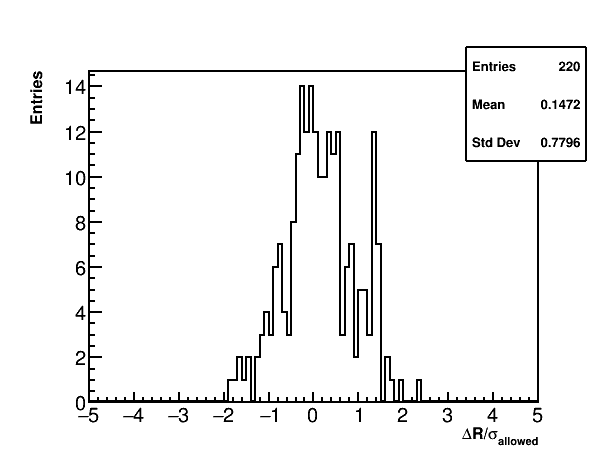
\includegraphics[width=0.65\textwidth]{AllSigmas}
\caption{Deviations between best-fit \R values for all datasets for the individual analysis comparisons. The entries from the top-right of the diagonal of Tables~\ref{tab:60h_diff} through \ref{tab:EG_diff} are taken and filled into this histogram. In general such a pull distribution should be a unit Gaussian, however entries from the same row or column will be correlated, so a perfect Gaussian is not expected. This is particularly apparent with the spike around $1.35\sigma$, which comes from some of the Q-Method correlations in the HK and 9d datasets, in both of which the Q-Method fits returned a greater \R-value than the rest of the methods.}
\label{fig:AllSigmas}
\end{figure}




\begin{landscape}
\begin{table}
\small
\centering
\renewcommand{\arraystretch}{1.5}
\begin{tabularx}{1\linewidth}{@{\extracolsep{\fill}}lXXXXXXXXXXX}
  \toprule
  	\multicolumn{12}{c}{{\normalsize 60h Analysis Differences}} \\
  \midrule
  	       & BU T & BU R & CU T & CU A & UW T & UW A & EU T & EU A & SJTU T & SJTU A & UK Q \\
  \midrule
	BU T   & 0.0000 $+0.00$ & 0.1154 $-1.42$ & 0.4495 $+1.32$ & 0.5943 $+0.96$ & 0.1555 $+1.17$ & 0.5983 $+0.28$ & 0.2817 $-0.29$ & 0.5890 $+0.55$ & 0.0609 $+1.03$ & 0.5781 $+0.66$ & 1.7692 $-0.23$  \\
	BU R   & 0.1154 $+1.42$ & 0.0000 $+0.00$ & 0.4609 $+1.64$ & 0.6015 $+1.23$ & 0.1464 $+2.37$ & 0.5963 $+0.55$ & 0.2862 $+0.29$ & 0.5912 $+0.82$ & 0.1288 $+1.76$ & 0.5867 $+0.93$ & 1.7731 $-0.14$  \\
	CU T   & 0.4495 $-1.32$ & 0.4609 $-1.64$ & 0.0000 $+0.00$ & 0.5710 $-0.03$ & 0.4642 $-0.88$ & 0.6017 $-0.71$ & 0.4628 $-1.46$ & 0.5933 $-0.46$ & 0.4484 $-1.18$ & 0.5854 $-0.36$ & 1.7710 $-0.56$  \\
	CU A   & 0.5943 $-0.96$ & 0.6015 $-1.23$ & 0.5710 $+0.03$ & 0.0000 $+0.00$ & 0.5879 $-0.67$ & 0.2172 $-1.88$ & 0.5813 $-1.13$ & 0.2050 $-1.23$ & 0.5846 $-0.87$ & 0.1774 $-1.09$ & 1.6581 $-0.59$  \\
	UW T   & 0.1555 $-1.17$ & 0.1464 $-2.37$ & 0.4642 $+0.88$ & 0.5879 $+0.67$ & 0.0000 $+0.00$ & 0.5619 $-0.03$ & 0.2851 $-0.93$ & 0.5731 $+0.24$ & 0.1600 $-0.75$ & 0.5741 $+0.34$ & 1.7583 $-0.33$  \\
	UW A   & 0.5983 $-0.28$ & 0.5963 $-0.55$ & 0.6017 $+0.71$ & 0.2172 $+1.88$ & 0.5619 $+0.03$ & 0.0000 $+0.00$ & 0.5767 $-0.43$ & 0.1419 $+1.10$ & 0.5888 $-0.17$ & 0.1572 $+1.36$ & 1.6580 $-0.34$  \\
	EU T   & 0.2817 $+0.29$ & 0.2862 $-0.29$ & 0.4628 $+1.46$ & 0.5813 $+1.13$ & 0.2851 $+0.93$ & 0.5767 $+0.43$ & 0.0000 $+0.00$ & 0.5553 $+0.73$ & 0.2827 $+0.51$ & 0.5696 $+0.81$ & 1.7456 $-0.18$  \\
	EU A   & 0.5890 $-0.55$ & 0.5912 $-0.82$ & 0.5933 $+0.46$ & 0.2050 $+1.23$ & 0.5731 $-0.24$ & 0.1419 $-1.10$ & 0.5553 $-0.73$ & 0.0000 $+0.00$ & 0.5786 $-0.45$ & 0.1389 $+0.42$ & 1.6580 $-0.44$  \\
	SJTU T & 0.0609 $-1.03$ & 0.1288 $-1.76$ & 0.4484 $+1.18$ & 0.5846 $+0.87$ & 0.1600 $+0.75$ & 0.5888 $+0.17$ & 0.2827 $-0.51$ & 0.5786 $+0.45$ & 0.0000 $+0.00$ & 0.5641 $+0.56$ & 1.7665 $-0.26$  \\
	SJTU A & 0.5781 $-0.66$ & 0.5867 $-0.93$ & 0.5854 $+0.36$ & 0.1774 $+1.09$ & 0.5741 $-0.34$ & 0.1572 $-1.36$ & 0.5696 $-0.81$ & 0.1389 $-0.42$ & 0.5641 $-0.56$ & 0.0000 $+0.00$ & 1.6632 $-0.47$  \\
	UK Q   & 1.7692 $+0.23$ & 1.7731 $+0.14$ & 1.7710 $+0.56$ & 1.6581 $+0.59$ & 1.7583 $+0.33$ & 1.6580 $+0.34$ & 1.7456 $+0.18$ & 1.6580 $+0.44$ & 1.7665 $+0.26$ & 1.6632 $+0.47$ & 0.0000 $+0.00$  \\
  \bottomrule
\end{tabularx}
\caption[]{Differences in results for the 60h dataset between the different analyses. The top number is the allowed ppb difference in \R, $\sigma_{\text{allowed}}$, as calculated from the correlation coefficients and analysis errors. The bottom number is the calculated deviation between analyses, calculated as $\sigma_{\text{dev}} = (R_{\text{column}}-R_{\text{row}})/\sigma_{\text{allowed}}$, where $R_{\text{column}}$ and $R_{\text{row}}$ come from \tabref{tab:analysisRValues} for the respective analyses.}
\label{tab:60h_diff}
\end{table}
\end{landscape}




\begin{landscape}
\begin{table}
\small
\centering
\renewcommand{\arraystretch}{1.5}
\begin{tabularx}{1\linewidth}{@{\extracolsep{\fill}}lXXXXXXXXXXX}
  \toprule
  	\multicolumn{12}{c}{{\normalsize HK Analysis Differences}} \\
  \midrule
  	       & BU T & BU R & CU T & CU A & UW T & UW A & EU T & EU A & SJTU T & SJTU A & UK Q \\
  \midrule
	BU T   & 0.0000 $+0.00$ & 0.0943 $-1.75$ & 0.3736 $-0.44$ & 0.5218 $+0.19$ & 0.1293 $+0.30$ & 0.5184 $+0.15$ & 0.2310 $-0.16$ & 0.5172 $+0.04$ & 0.0544 $+0.78$ & 0.5094 $-0.09$ & 1.5421 $+1.36$  \\
	BU R   & 0.0943 $+1.75$ & 0.0000 $+0.00$ & 0.3846 $-0.00$ & 0.5262 $+0.50$ & 0.1256 $+1.63$ & 0.5153 $+0.47$ & 0.2389 $+0.54$ & 0.5172 $+0.36$ & 0.1087 $+1.91$ & 0.5143 $+0.23$ & 1.5454 $+1.46$  \\
	CU T   & 0.3736 $+0.44$ & 0.3846 $+0.00$ & 0.0000 $+0.00$ & 0.5015 $+0.52$ & 0.3891 $+0.53$ & 0.5267 $+0.46$ & 0.3878 $+0.33$ & 0.5246 $+0.36$ & 0.3724 $+0.56$ & 0.5169 $+0.23$ & 1.5470 $+1.46$  \\
	CU A   & 0.5218 $-0.19$ & 0.5262 $-0.50$ & 0.5015 $-0.52$ & 0.0000 $+0.00$ & 0.5208 $-0.11$ & 0.1842 $-0.10$ & 0.5114 $-0.26$ & 0.1788 $-0.42$ & 0.5119 $-0.11$ & 0.1502 $-0.96$ & 1.4443 $+1.38$  \\
	UW T   & 0.1293 $-0.30$ & 0.1256 $-1.63$ & 0.3891 $-0.53$ & 0.5208 $+0.11$ & 0.0000 $+0.00$ & 0.4934 $+0.08$ & 0.2380 $-0.32$ & 0.5080 $-0.03$ & 0.1338 $+0.02$ & 0.5101 $-0.17$ & 1.5328 $+1.34$  \\
	UW A   & 0.5184 $-0.15$ & 0.5153 $-0.47$ & 0.5267 $-0.46$ & 0.1842 $+0.10$ & 0.4934 $-0.08$ & 0.0000 $+0.00$ & 0.5022 $-0.23$ & 0.1181 $-0.47$ & 0.5086 $-0.07$ & 0.1314 $-0.95$ & 1.4438 $+1.40$  \\
	EU T   & 0.2310 $+0.16$ & 0.2389 $-0.54$ & 0.3878 $-0.33$ & 0.5114 $+0.26$ & 0.2380 $+0.32$ & 0.5022 $+0.23$ & 0.0000 $+0.00$ & 0.4888 $+0.12$ & 0.2301 $+0.34$ & 0.5004 $-0.02$ & 1.5251 $+1.40$  \\
	EU A   & 0.5172 $-0.04$ & 0.5172 $-0.36$ & 0.5246 $-0.36$ & 0.1788 $+0.42$ & 0.5080 $+0.03$ & 0.1181 $+0.47$ & 0.4888 $-0.12$ & 0.0000 $+0.00$ & 0.5064 $+0.04$ & 0.1163 $-0.60$ & 1.4439 $+1.44$  \\
	SJTU T & 0.0544 $-0.78$ & 0.1087 $-1.91$ & 0.3724 $-0.56$ & 0.5119 $+0.11$ & 0.1338 $-0.02$ & 0.5086 $+0.07$ & 0.2301 $-0.34$ & 0.5064 $-0.04$ & 0.0000 $+0.00$ & 0.4956 $-0.18$ & 1.5365 $+1.34$  \\
	SJTU A & 0.5094 $+0.09$ & 0.5143 $-0.23$ & 0.5169 $-0.23$ & 0.1502 $+0.96$ & 0.5101 $+0.17$ & 0.1314 $+0.95$ & 0.5004 $+0.02$ & 0.1163 $+0.60$ & 0.4956 $+0.18$ & 0.0000 $+0.00$ & 1.4472 $+1.48$  \\
	UK Q   & 1.5421 $-1.36$ & 1.5454 $-1.46$ & 1.5470 $-1.46$ & 1.4443 $-1.38$ & 1.5328 $-1.34$ & 1.4438 $-1.40$ & 1.5251 $-1.40$ & 1.4439 $-1.44$ & 1.5365 $-1.34$ & 1.4472 $-1.48$ & 0.0000 $+0.00$  \\
  \bottomrule
\end{tabularx}
\caption[]{Differences in results for the HK dataset between the different analyses. The top number is the allowed ppb difference in \R, $\sigma_{\text{allowed}}$, as calculated from the correlation coefficients and analysis errors. The bottom number is the calculated deviation between analyses, calculated as $\sigma_{\text{dev}} = (R_{\text{column}}-R_{\text{row}})/\sigma_{\text{allowed}}$, where $R_{\text{column}}$ and $R_{\text{row}}$ come from \tabref{tab:analysisRValues} for the respective analyses.}
\label{tab:HK_diff}
\end{table}
\end{landscape}



\begin{landscape}
\begin{table}
\small
\centering
\renewcommand{\arraystretch}{1.5}
\begin{tabularx}{1\linewidth}{@{\extracolsep{\fill}}lXXXXXXXXXXX}
  \toprule
  	\multicolumn{12}{c}{{\normalsize 9d Analysis Differences}} \\
  \midrule
  	       & BU T & BU R & CU T & CU A & UW T & UW A & EU T & EU A & SJTU T & SJTU A & UK Q \\
  \midrule
	BU T   & 0.0000 $+0.00$ & 0.0775 $-0.06$ & 0.3076 $-0.34$ & 0.4220 $+0.86$ & 0.1040 $+0.17$ & 0.4177 $+0.83$ & 0.1911 $+0.15$ & 0.4148 $+0.76$ & 0.0415 $+0.57$ & 0.4088 $+0.42$ & 1.2432 $+1.32$  \\
	BU R   & 0.0775 $+0.06$ & 0.0000 $+0.00$ & 0.3164 $-0.31$ & 0.4281 $+0.86$ & 0.1007 $+0.23$ & 0.4171 $+0.84$ & 0.1940 $+0.17$ & 0.4174 $+0.77$ & 0.0874 $+0.32$ & 0.4149 $+0.43$ & 1.2487 $+1.32$  \\
	CU T   & 0.3076 $+0.34$ & 0.3164 $+0.31$ & 0.0000 $+0.00$ & 0.3974 $+1.18$ & 0.3175 $+0.38$ & 0.4156 $+1.08$ & 0.3100 $+0.42$ & 0.4151 $+1.01$ & 0.3052 $+0.42$ & 0.4083 $+0.68$ & 1.2334 $+1.41$  \\
	CU A   & 0.4220 $-0.86$ & 0.4281 $-0.86$ & 0.3974 $-1.18$ & 0.0000 $+0.00$ & 0.4213 $-0.82$ & 0.1513 $-0.13$ & 0.4130 $-0.81$ & 0.1469 $-0.32$ & 0.4139 $-0.82$ & 0.1241 $-1.54$ & 1.1522 $+1.11$  \\
	UW T   & 0.1040 $-0.17$ & 0.1007 $-0.23$ & 0.3175 $-0.38$ & 0.4213 $+0.82$ & 0.0000 $+0.00$ & 0.3978 $+0.82$ & 0.1948 $+0.05$ & 0.4085 $+0.73$ & 0.1067 $+0.05$ & 0.4089 $+0.38$ & 1.2327 $+1.31$  \\
	UW A   & 0.4177 $-0.83$ & 0.4171 $-0.84$ & 0.4156 $-1.08$ & 0.1513 $+0.13$ & 0.3978 $-0.82$ & 0.0000 $+0.00$ & 0.4019 $-0.79$ & 0.0973 $-0.28$ & 0.4100 $-0.78$ & 0.1031 $-1.67$ & 1.1483 $+1.13$  \\
	EU T   & 0.1911 $-0.15$ & 0.1940 $-0.17$ & 0.3100 $-0.42$ & 0.4130 $+0.81$ & 0.1948 $-0.05$ & 0.4019 $+0.79$ & 0.0000 $+0.00$ & 0.3912 $+0.74$ & 0.1911 $-0.02$ & 0.4002 $+0.36$ & 1.2332 $+1.31$  \\
	EU A   & 0.4148 $-0.76$ & 0.4174 $-0.77$ & 0.4151 $-1.01$ & 0.1469 $+0.32$ & 0.4085 $-0.73$ & 0.0973 $+0.28$ & 0.3912 $-0.74$ & 0.0000 $+0.00$ & 0.4062 $-0.72$ & 0.0900 $-1.60$ & 1.1532 $+1.14$  \\
	SJTU T & 0.0415 $-0.57$ & 0.0874 $-0.32$ & 0.3052 $-0.42$ & 0.4139 $+0.82$ & 0.1067 $-0.05$ & 0.4100 $+0.78$ & 0.1911 $+0.02$ & 0.4062 $+0.72$ & 0.0000 $+0.00$ & 0.3982 $+0.38$ & 1.2417 $+1.30$  \\
	SJTU A & 0.4088 $-0.42$ & 0.4149 $-0.43$ & 0.4083 $-0.68$ & 0.1241 $+1.54$ & 0.4089 $-0.38$ & 0.1031 $+1.67$ & 0.4002 $-0.36$ & 0.0900 $+1.60$ & 0.3982 $-0.38$ & 0.0000 $+0.00$ & 1.1581 $+1.26$  \\
	UK Q   & 1.2432 $-1.32$ & 1.2487 $-1.32$ & 1.2334 $-1.41$ & 1.1522 $-1.11$ & 1.2327 $-1.31$ & 1.1483 $-1.13$ & 1.2332 $-1.31$ & 1.1532 $-1.14$ & 1.2417 $-1.30$ & 1.1581 $-1.26$ & 0.0000 $+0.00$  \\
  \bottomrule
\end{tabularx}
\caption[]{Differences in results for the 9d dataset between the different analyses. The top number is the allowed ppb difference in \R, $\sigma_{\text{allowed}}$, as calculated from the correlation coefficients and analysis errors. The bottom number is the calculated deviation between analyses, calculated as $\sigma_{\text{dev}} = (R_{\text{column}}-R_{\text{row}})/\sigma_{\text{allowed}}$, where $R_{\text{column}}$ and $R_{\text{row}}$ come from \tabref{tab:analysisRValues} for the respective analyses.}
\label{tab:9d_diff}
\end{table}
\end{landscape}




\begin{landscape}
\begin{table}
\small
\centering
\renewcommand{\arraystretch}{1.5}
\begin{tabularx}{1\linewidth}{@{\extracolsep{\fill}}lXXXXXXXXXXX}
  \toprule
  	\multicolumn{12}{c}{{\normalsize EG Analysis Differences}} \\
  \midrule
  	       & BU T & BU R & CU T & CU A & UW T & UW A & EU T & EU A & SJTU T & SJTU A & UK Q \\
  \midrule
	BU T   & 0.0000 $+0.00$ & 0.0602 $-1.05$ & 0.2421 $-0.05$ & 0.3325 $+0.34$ & 0.0806 $-0.15$ & 0.3256 $+0.10$ & 0.1461 $-1.20$ & 0.3266 $-0.08$ & 0.0346 $+1.04$ & 0.3226 $+0.02$ & 1.0990 $-0.26$  \\
	BU R   & 0.0602 $+1.05$ & 0.0000 $+0.00$ & 0.2495 $+0.20$ & 0.3372 $+0.52$ & 0.0781 $+0.65$ & 0.3257 $+0.29$ & 0.1513 $-0.74$ & 0.3282 $+0.12$ & 0.0687 $+1.45$ & 0.3276 $+0.22$ & 1.1029 $-0.20$  \\
	CU T   & 0.2421 $+0.05$ & 0.2495 $-0.20$ & 0.0000 $+0.00$ & 0.3100 $+0.40$ & 0.2497 $+0.00$ & 0.3221 $+0.14$ & 0.2464 $-0.66$ & 0.3215 $-0.04$ & 0.2409 $+0.21$ & 0.3188 $+0.07$ & 1.0972 $-0.25$  \\
	CU A   & 0.3325 $-0.34$ & 0.3372 $-0.52$ & 0.3100 $-0.40$ & 0.0000 $+0.00$ & 0.3337 $-0.37$ & 0.1183 $-0.67$ & 0.3270 $-0.88$ & 0.1122 $-1.22$ & 0.3274 $-0.23$ & 0.1012 $-1.03$ & 1.0387 $-0.39$  \\
	UW T   & 0.0806 $+0.15$ & 0.0781 $-0.65$ & 0.2497 $-0.00$ & 0.3337 $+0.37$ & 0.0000 $+0.00$ & 0.3125 $+0.14$ & 0.1505 $-1.08$ & 0.3230 $-0.04$ & 0.0851 $+0.57$ & 0.3249 $+0.06$ & 1.0960 $-0.25$  \\
	UW A   & 0.3256 $-0.10$ & 0.3257 $-0.29$ & 0.3221 $-0.14$ & 0.1183 $+0.67$ & 0.3125 $-0.14$ & 0.0000 $+0.00$ & 0.3182 $-0.65$ & 0.0751 $-0.77$ & 0.3204 $+0.01$ & 0.0816 $-0.31$ & 1.0406 $-0.31$  \\
	EU T   & 0.1461 $+1.20$ & 0.1513 $+0.74$ & 0.2464 $+0.66$ & 0.3270 $+0.88$ & 0.1505 $+1.08$ & 0.3182 $+0.65$ & 0.0000 $+0.00$ & 0.3115 $+0.48$ & 0.1460 $+1.45$ & 0.3193 $+0.57$ & 1.0964 $-0.10$  \\
	EU A   & 0.3266 $+0.08$ & 0.3282 $-0.12$ & 0.3215 $+0.04$ & 0.1122 $+1.22$ & 0.3230 $+0.04$ & 0.0751 $+0.77$ & 0.3115 $-0.48$ & 0.0000 $+0.00$ & 0.3208 $+0.19$ & 0.0746 $+0.44$ & 1.0437 $-0.25$  \\
	SJTU T & 0.0346 $-1.04$ & 0.0687 $-1.45$ & 0.2409 $-0.21$ & 0.3274 $+0.23$ & 0.0851 $-0.57$ & 0.3204 $-0.01$ & 0.1460 $-1.45$ & 0.3208 $-0.19$ & 0.0000 $+0.00$ & 0.3145 $-0.09$ & 1.0977 $-0.30$  \\
	SJTU A & 0.3226 $-0.02$ & 0.3276 $-0.22$ & 0.3188 $-0.07$ & 0.1012 $+1.03$ & 0.3249 $-0.06$ & 0.0816 $+0.31$ & 0.3193 $-0.57$ & 0.0746 $-0.44$ & 0.3145 $+0.09$ & 0.0000 $+0.00$ & 1.0411 $-0.28$  \\
	UK Q   & 1.0990 $+0.26$ & 1.1029 $+0.20$ & 1.0972 $+0.25$ & 1.0387 $+0.39$ & 1.0960 $+0.25$ & 1.0406 $+0.31$ & 1.0964 $+0.10$ & 1.0437 $+0.25$ & 1.0977 $+0.30$ & 1.0411 $+0.28$ & 0.0000 $+0.00$  \\
  \bottomrule
\end{tabularx}
\caption[]{Differences in results for the EG dataset between the different analyses. The top number is the allowed ppb difference in \R, $\sigma_{\text{allowed}}$, as calculated from the correlation coefficients and analysis errors. The bottom number is the calculated deviation between analyses, calculated as $\sigma_{\text{dev}} = (R_{\text{column}}-R_{\text{row}})/\sigma_{\text{allowed}}$, where $R_{\text{column}}$ and $R_{\text{row}}$ come from \tabref{tab:analysisRValues} for the respective analyses.}
\label{tab:EG_diff}
\end{table}
\end{landscape}





